\documentclass[tikz,border=2pt]{standalone}
\usepackage{tikz}
\usepackage[european]{circuitikz}
\usetikzlibrary{arrows.meta,positioning,calc}
../cictikz/src/cictikz/data/tex/cictikz_lib.tex
\begin{document}
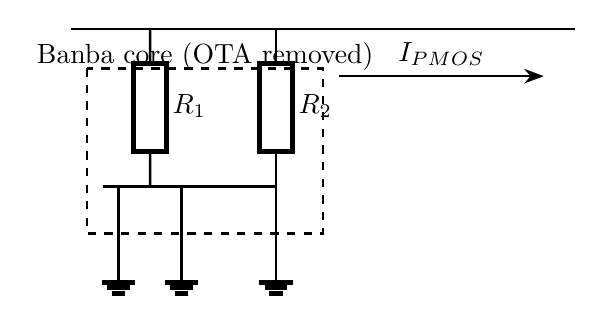
\begin{tikzpicture}[>=Stealth, line width=0.9pt]
  \draw (0,3.0) -- (6.4,3.0);
  \draw (1.0,3.0) to[resistor,l=$R_1$] (1.0,1.0);
  \draw (2.6,3.0) to[resistor,l=$R_2$] (2.6,1.0);
  \draw (0.4,1.0) -- (2.6,1.0);
  \draw (0.6,1.0) -- (0.6,0.2) node[ground] {};
  \draw (1.4,1.0) -- (1.4,0.2) node[ground] {};
  \draw (2.6,1.0) -- (2.6,0.2) node[ground] {};
  \draw[dashed] (0.2,2.5) rectangle (3.2,0.4);
  \node at (1.7,2.65) {Banba core (OTA removed)};
  \draw[->] (3.4,2.4) -- (6.0,2.4) node[midway,above] {$I_{PMOS}$};
\end{tikzpicture}
\end{document}
